%===================================================================================================
\subsection{Wider Population: Bias Adjustment}\label{mod.par.wp}
We stratified the remaining women and men (besides FSW and clients)
by numbers of partners in the past 12 months (p12m): 0--1 and 2+.
The 2006-07 DHS \cite{SDHS2006}, 2011 SHIMS \cite{SHIMS1}, and 2016-17 SHIMS2 \cite{SHIMS2} surveys
provide the numbers of respondents who reported 2+ partners in the past 12 months (p12m):
13.5, 18.2, 14.5\% among men, and 1.6, 3.8, 4.1\% among women, respectively.%
\footnote{From
  Tables~14.7.1 and 14.7.2 (ages 15-49) in \cite{SDHS2006},
  Table~3 (ages 18-49) in \cite{SHIMS1},
  Table~15.3.A (ages 15+) in \cite{SHIMS2},
  with manual adjustment for survey skip patterns in \cite{SDHS2006,SHIMS2}.}
However, such reports are likely substantially biased by
social desirability bias due to the face-to-face interview format
\cite{Konings1995,Plummer2004,Gregson2004,Behanzin2013}.
Moreover, these data do not provide information on the \emph{types} of partners reported
--- \ie those reporting 1 partner in p12m
are not necessarily in a main/spousal (vs casual) partnership,
and neither are those reporting 2+ partners in p12m.
Here we develop and apply a new method to adjust for these potential reporting biases,
and simultaneously estimate the numbers of main/spousal and casual partners among each stratum.
The results of these analyses then directly inform
activity group sizes in \sref{mod.par.size.wp} and
numbers of partners in \sref{mod.par.pnum.mcx}.
%---------------------------------------------------------------------------------------------------
\subsubsection{Reported Partner Numbers}\label{mod.par.wp.data}
Both the 2006 DHS \cite[Tables 14.6.1 and 14.6.2]{SDHS2006}
and 2016-17 SHIMS \cite[Tables 15.4.A and 15.4.B]{SHIMS2}
summarize the numbers of women and men by partners in p12m \emph{and} by marital/union status,
but summaries are stratified by each factor separately, not jointly.
However, making the following assumptions,
we estimated the jointly-stratified proportions of individuals.
Let $W_{2+}$, $W_{1}$, and $W_{0}$ denote women reporting 2+, 1, and 0 partners, respectively,
and likewise with $M_{2+}$, $M_{1}$, $M_{0}$ for men (all partners reflect p12m).
The assumptions were:
\begin{itemize}
  \item $W_{2+}$ included all women in non-polygynous unions (married or cohabiting)
  reporting sex with a ``casual'' (non-marital, non-cohabiting) partner
  \item $M_{2+}$ included all men in polygynous unions,
  plus all men in non-polygynous unions reporting sex with a casual partner
  \item the remaining $W_{2+}$ and $M_{2+}$ formed only casual partnerships
  \item all women and men in non-polygynous unions
  reporting no sex with a casual partner reported 1 partner ($W_{1}$ and $M_{1}$)
  \item the remaining $W_{1}$ and $M_{1}$ formed only casual partnerships
\end{itemize}
Figure~\ref{fig:xwp} illustrates the resulting
proportions of women and men in each union / partners in p12m stratum
in 2006-07 \sfref{fig:xwp.2006} and 2016-17 \sfref{fig:xwp.2016}.
\begin{figure}
  \centering
  \begin{subfigure}{0.7\linewidth}
    \centering
    \includegraphics[width=\linewidth]{xwp.2006}
    \caption{2006-07 \cite{SDHS2006}}
    \label{fig:xwp.2006}
  \end{subfigure}
  \begin{subfigure}{0.7\linewidth}
    \centering
    \includegraphics[width=\linewidth]{xwp.2016}
    \caption{2016 \cite{SHIMS2}}
    \label{fig:xwp.2016}
  \end{subfigure}
  \begin{subfigure}{0.7\linewidth}
    \centering
    \includegraphics[width=\linewidth]{xwp.adj}
    \caption{Adjusted (mean)}
    \label{fig:xwp.adj}
  \end{subfigure}
  \caption{Reported proportions of women and men aged 15--49,
    stratified by union status and numbers of partners in the past 12 months}
  \label{fig:xwp}
\end{figure}
%---------------------------------------------------------------------------------------------------
\subsubsection{Bias Adjustment: Rationale}\label{mod.par.wp.rat}
We were motivated to examine potential reporting bias because
$M_{2+}$ is consistently much greater than $W_{2+}$.
In fact, this difference is common in surveys \cite{Todd2009,Higgins2010},
and could be explained by either:
(a) a small number of women with many partners,
such as FSW, who may also not be reached by the survey,
or who may not fully report partner numbers;
(b) over-reporting of partnerships by men; or
(c) under-reporting of partnerships by women.
Further stratification of women reporting 2+ partners in \cite[Table~14.7.1]{SDHS2006}
revealed that 94\% reported exactly 2 whereas 6\% reported 3+,
suggesting that explanation (a) is less likely unless
women with 3+ partners are under-reported or indeed missing from the survey.
\par
\citet{Gregson2002bias} (Zimbabwe), \citet{Nnko2004} (Tanzania) and \citet{Clark2011} (Kenya)
explored explanations (b) and (c) through measures of consistency; their results suggested that
under-reporting of non-spousal partnerships by women (c) was more likely,
perhaps due to social norms and pressures.
Such norms in Eswatini are explored in \cite{Ruark2014,Fielding-Miller2016,Ruark2019,Pulerwitz2021}.
In fact, a review comparing computer-based tools \vs face-to-face interviews
for surveying sexual behaviour \cite{Langhaug2010} found that
\emph{both} women and men may under-report sexual partners, but women more so.
A notable 2008 study in Benin \cite{Behanzin2013} found that
7 times as many married women (21 \vs 3\%) and 3 times as many married men (53 \vs 18\%)
reported any extramarital sex in p12m
in a survey via anonymous polling booth \vs face-to-face interview.
Similarly, 5 times as many unmarried women (13.5 \vs 2.8\%) reported
exchanging sex for money, gifts or favours in p12m, while
4 times as many unmarried men (62 \vs 14\%) reported non-transactional sex with a women in p12m.
Such findings were similar to those from Zimbabwe (1990s) \cite{Gregson2002bias}.
%---------------------------------------------------------------------------------------------------
\subsubsection{Bias Adjustment: Approach}\label{mod.par.wp.appr}
To account for the above potential reporting biases
and qualitative insights from \cite{Ruark2014,Fielding-Miller2016,Ruark2019,Pulerwitz2021},
We modelled the adjusted proportions of Swati women and men
in each union / partners in p12m stratum as follows.
Let $W_{s1}$ and $W_{u1}$ denote sub-proportions of $W_{1}$ who are single and in a union, respectively,
and likewise for $W_{s2+}$, $W_{u2+}$, $M_{s1}$, $M_{u1}$, $M_{s2+}$, and $M_{u2+}$.
Further, let $W_{s1}$ denote the reported proportion of women (average of 2006-07 and 2016-17),
\vs $W'_{s1}$ denoting the adjusted proportion.
We assumed that a faction of $W_{0}$ belongs in $W'_{s1}$
--- \ie a fraction of women reporting 0 partners in p12m truly had 1 casual (non-main/spousal) partner.
We modelled this relationship through an odds ratio $\varphi_{W,s1:0}$,
which is roughly equivalent in interpretation to
the proportion ratios estimated by \citet{Behanzin2013}:%
\footnote{Odds ratios ensure no proportions become greater than one or negative.}
\begin{equation}\label{eq:wp.or}
  \varphi_{Ws1:0} = \frac{W'_{s1}}{W'_{0}} \bigg/ \frac{W_{s1}}{W_{0}}
\end{equation}
We defined similar odds ratios $\varphi_{Ws2+:s1}$, $\varphi_{Wu2+:u1}$,
$\varphi_{Wu1:0}$, $\varphi_{Wu1:s1}$, and $\varphi_{Wu2+:s2+}$, and likewise for men.
These strata and the corresponding adjustments / reallocations of women
from reported to adjusted strata are illustrated in Figure~\ref{fig:model.nsw.adj}.
To resolve the adjusted values $W'$ then requires
solving the (nonlinear) system of 6 equations corresponding to the 6 odds ratios $\varphi$,
subject to $\sum_i W'_i = 1$ and $0 \le W'_i < 1$.
An exact solution is not guaranteed,
but the sum squared error from all equations can be minimized.
The odds ratios $\varphi$ were then defined as follows, including sampling distributions.
\begin{figure}
  \centering
  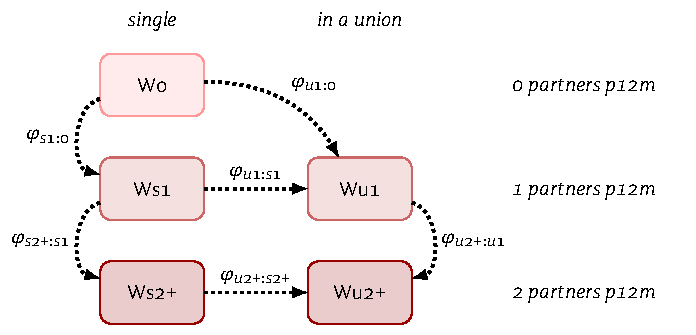
\includegraphics[scale=.8]{diag.nsw.adj}
  \caption{Illustration of how the proportions of women (and equivalently men)
    are adjusted / reallocated between union / partners in p12m strata
    based on odds ratios $\varphi$}
  \label{fig:model.nsw.adj}
  \floatfoot{
    p12m: within the past 12 months;
    W0: 0 partners in p12m;
    Ws1: single (not married/cohabiting) and 1 partner in p12m;
    Wu1: in a union (married/cohabiting) and 1 partner in p12m;
    Ws2+: single and 2+ partners in p12m;
    Wu2+: in a union and 2+ partners in p12m.
    $\varphi$: odds of truly being in the second (arrowhead) \vs first (tail) group.}
\end{figure}
%---------------------------------------------------------------------------------------------------
\paragraph{Union Status}
We assumed that under-reporting of main/spousal partnerships was minimal,
but that some ``main'' partnerships may not be captured in
the definition ``married/cohabiting'' from \cite{SDHS2006,SHIMS2};
thus $\varphi_{u1:0}$, $\varphi_{u1:s1}$, and $\varphi_{u2+:s2+}$
would be small but greater than 1
(horizontal transitions in Figure~\ref{fig:model.nsw.adj}).
Moreover, based on the median age of marriage, 23--29 \cite{SDHS2006},
approximately half of respondents aged 15--49 would have been married,
whereas only 28--39\% of women and men reported being in a union
(Figure~\ref{fig:xwp.2006}~and~\ref{fig:xwp.2016}),
although some marriages end in divorce/widowing \cite{SDHS2006}.
Thus, we sampled each of $\varphi_{u1:0}$, $\varphi_{u1:s1}$, and $\varphi_{u2+:s2+}$
from $1+\opname{Gamma}(\alpha,\beta=1)$
with $\alpha=.5$ for women and $\alpha=.3$ for men,
yielding mean (95\%~CI): 1.50~(1.00,~3.51) and 1.30~(1.00,~2.90), respectively.
%---------------------------------------------------------------------------------------------------
\paragraph{Partner Numbers}
Next, regarding partner numbers,
we defined $\varphi_{s1:0}$, $\varphi_{s2+:s1}$, and $\varphi_{u2+:u1}$ as follows
(vertial transitions in Figure~\ref{fig:model.nsw.adj}).
The median age of first sex in Eswatini was
approximately 18 for women and 19.5 for men \cite{SDHS2006}.
Thus, the 31--36\% of women and 34--41\% of men aged 15--49 reporting no partners in p12m
(Figure~\ref{fig:xwp.2006}~and~\ref{fig:xwp.2016}) is likely overestimated,
although some individuals may be abstinent in p12m following sexual debut.
We assumed that women had 3 and men had 2 times the odds of
actually having 1 casual partner in p12m while reporting no partners.
Thus, we sampled $\varphi_{s1:0}$ from $1+\opname{Gamma}(\alpha,\beta=1)$
with $\alpha=2$ for women and $\alpha=1$ for men,
yielding mean (95\%~CI): 3.00~(1.24,~6.57) and 2.00~(1.03,~4.69), respectively.
Drawing on \cite{Behanzin2013}, we assumed that ``single'' women and men (not married/cohabiting)
were less likely to report multiple partners in p12m, but women more so.
Thus, we sampled $\varphi_{s2+:s1}$ from $1+\opname{Gamma}(\alpha,\beta=1)$
with $\alpha=4$ for women and $\alpha=1$ for men,
yielding 5.00~(2.09,~9.77) and 2.00~(1.03,~4.69).
We made a similar assumption about married/cohabiting women and men,
with the same odds for men, but even greater odds of non-reporting among women.
We sampled $\varphi_{u2+:u1}$ from $1+\opname{Gamma}(\alpha,\beta=1)$
with $\alpha=6$ for women and $\alpha=1$ for men,
yielding 7.00~(3.20,~12.67) and 2.00~(1.03,~4.69).
%---------------------------------------------------------------------------------------------------
\subsubsection{Bias Adjustment: Results}\label{mod.par.wp.res}
The mean resulting adjusted proportions $W'$ and $M'$
from solving the system with the assumed odds ratios $\varphi$
are illustrated in Figure~\ref{fig:xwp.adj}, which can be compared to
the reported proportions in \sfref{fig:xwp.2006}~and~\sfref{fig:xwp.2016}.
Figure~\ref{fig:xwp.adj.dens} also illustrates the empiric density distributions
for each element $W'_{i}$ and $M'_{i}$.
Numerically, the mean (95\%~CI) estimates were:
\begin{itemize}
  \item $W'_{0} = 17~(9,~27)$\% of women and $M'_{0} = 25~(13,~35)\%$ of men had 0 partners in p12m
  \item $W'_{1} = 66~(57,~75)$\% of women and $M'_{1} = 49~(37,~61)\%$ of men had 1 partners in p12m
  \item $W'_{2+} = 17~(10,~27)$\% of women and $M'_{2+} = 26~(15,~44)$\% of men had 2+ partners in p12m
  \item $W'_{u1} / W'_{01} = 38~(21,57)$\% women and $M'_{u1} / M'_{01} = 35~(23,~50)$\% men
    with 0--1 partners in p12m were in a main/spousal partnership
  \item $W'_{s1} / W'_{01} = 41~(19,65)$\% women and $M'_{s1} / M'_{01} = 31~(15,~55)$\% men
    with 0--1 partners in p12m were in a single casual partnership
  \item $W'_{u2+} / W'_{2+} = 32~(9,55)$\% women and $M'_{u2+} / M'_{2+} = 38~(13,~62)$\% men
    with 2+ partners in p12m were in a main/spousal partnership,
    and the rest had only casual partnerships.
\end{itemize}
\begin{figure}
  \centering
  \includegraphics[width=.8\linewidth]{xwp.adj.distr}
  \caption{Density distributions for adjusted proportions of women and men aged 15--49,
    stratified by union status and numbers of partners in the past 12 months}
  \label{fig:xwp.adj.dens}
\end{figure}
